\chapter{Contexte général du projet}

\section{Introduction}
Ce premier chapitre décrit le contexte général du projet \textbf{Certif-fun}, en élaborant une étude approfondie des enjeux de la certification numérique et des besoins du secteur éducatif moderne. Nous mettrons en lumière les insuffisances des solutions actuelles afin de justifier les objectifs de ce travail. Enfin, nous présenterons la méthodologie de gestion de projet adoptée, basée sur le cadre Scrum, ainsi que la planification détaillée des tâches pour assurer une organisation optimale de la réalisation.

\section{Présentation du projet}
\subsection{Sujet du projet}
Le projet porte sur le développement de \textbf{Certif-fun}, une plateforme web intelligente de nouvelle génération dédiée à la gestion des certifications, à la surveillance automatisée (\textit{AI Proctoring}), à l'encadrement structuré et à la génération de contenu pédagogique par intelligence artificielle. 

Le système repose sur une architecture microservices robuste (Spring Boot, React, FastAPI) et intègre des technologies de pointe : 
\begin{itemize}
    \item \textbf{Vision par ordinateur :} Utilisation de YOLOv8 et MediaPipe pour le suivi en temps réel des comportements lors des examens.
    \item \textbf{IA Générative :} Intégration d'Ollama pour permettre aux formateurs de générer automatiquement des supports de cours et des quiz interactifs à partir de documents bruts.
    \item \textbf{Collaboration :} Espaces de visioconférence et modules d'encadrement pour un suivi personnalisé et proactif des apprenants.
\end{itemize}

Ce projet vise à transformer l'expérience éducative en fournissant un écosystème sécurisé et productif, réduisant la charge de travail administrative tout en garantissant l'intégrité académique.

\subsection{Intérêt du projet}
Ce projet présente plusieurs avantages stratégiques :
\begin{itemize}
    \item \textbf{Optimisation de la productivité :} La génération automatisée de contenus par IA libère les formateurs des tâches répétitives de création d'évaluations.
    \item \textbf{Sécurisation des certifications :} Le proctoring automatisé remplace la surveillance humaine coûteuse et sujette aux erreurs, garantissant un mérite authentique.
    \item \textbf{Suivi personnalisé et humain :} Malgré la distance, les outils de visioconférence et de gestion de tâches maintiennent un lien étroit entre formateur et apprenant.
    \item \textbf{Gain de temps et d'efficacité :} L'unification de tous ces outils dans une seule plateforme évite la fragmentation et simplifie la prise en main pour les institutions.
\end{itemize}

\section{Problématique et état de l’existant}
Face à la généralisation des formations à distance, une question centrale se pose : comment concevoir une plateforme unifiée capable de garantir à la fois l'intégrité des examens en ligne, la crédibilité des certifications délivrées, et une expérience fluide pour les formateurs comme pour les apprenants ?

En examinant ce qui existe aujourd'hui, on peut distinguer trois grandes approches pour la gestion et la sécurisation des examens en ligne :
\begin{itemize}
    \item \textbf{Les plateformes pédagogiques classiques} (comme Moodle ou Canvas) : elles assurent correctement la diffusion de contenus et le suivi des apprenants, mais traitent la sécurité des examens comme un problème extérieur, se limitant à des quiz simples sans vraiment contrôler les conditions de passation.
    \item \textbf{Les logiciels de surveillance spécialisés} (greffés sur ces plateformes) : ils enregistrent la webcam et verrouillent le navigateur, mais restent des ajouts externes qui créent des frictions techniques et dégradent l'expérience utilisateur.
    \item \textbf{La supervision humaine à distance} (un surveillant observe les étudiants via webcam) : bien que plus fiable en apparence, cette méthode est difficile à tenir à grande échelle en raison de la fatigue, de l'erreur humaine et du coût logistique.
\end{itemize}

Ces trois approches partagent des failles communes que \textbf{Certif-fun} cherche précisément à combler :
\begin{itemize}
    \item \textbf{L'absence de vérification de l'apprenant} : aucune solution ne s'assure réellement que la personne qui passe l'examen est bien celle qui s'est inscrite, laissant la porte ouverte à toute forme de substitution.
    \item \textbf{La surveillance fragmentée} : limitée à la vidéo, les outils actuels ne croisent pas simultanément plusieurs signaux tels que l'absence prolongée, le bruit ambiant ou le détournement du regard.
    \item \textbf{La dispersion des outils} : les formateurs et les étudiants doivent jongler entre plusieurs plateformes sans lien entre elles, ce qui nuit à la concentration et alourdit considérablement la gestion administrative.
\end{itemize}

\section{Objectifs du projet}
Les objectifs de Certif-fun s'articulent autour de trois dimensions :

\subsection{Objectifs Fonctionnels}
\begin{itemize}
    \item \textbf{Surveillance intelligente :} Détection automatique de fraude (présence de téléphone, absence, tiers, etc.).
    \item \textbf{Génération de contenu :} Création instantanée de quiz et de résumés de cours via LLMs.
    \item \textbf{Espace Collaboratif :} Système de visioconférence intégré et module de suivi de progression structuré.
    \item \textbf{Multi-portails :} Interfaces dédiées pour l'Admin, le Formateur et l'Apprenant.
\end{itemize}

\subsection{Objectifs Techniques}
\begin{itemize}
    \item \textbf{Architecture Microservices :} Conception d'une infrastructure modulaire et découplée pour garantir l'indépendance des services métier.
    \item \textbf{Performance temps réel :} Analyse vidéo fluide avec un temps de traitement minimal (inférieur à 1s).
    \item \textbf{Sécurité :} Authentification sécurisée par JWT et protection des données personnelles.
    \item \textbf{Modernité :} Utilisation de Spring Boot, React, FastAPI et Docker.
\end{itemize}

\subsection{Objectifs Pédagogiques}
\begin{itemize}
    \item Réduire le décrochage académique par un suivi plus réactif.
    \item Valoriser les diplômes par des certifications hautement sécurisées.
    \item Encourager l'autonomie de l'apprenant via des outils d'auto-évaluation.
\end{itemize}

\section{Démarche de gestion de projet}
\subsection{Choix de la méthode de gestion du projet}
Pour assurer la flexibilité et la réactivité face aux défis techniques de l'IA, nous avons adopté la méthodologie \textbf{Scrum} \cite{nacih2023scrum}. Ce cadre agile permet une livraison incrémentale des fonctionnalités et une adaptation continue aux besoins des utilisateurs finaux.

La figure \ref{fig:scrum_process} présente le schéma du cycle Scrum et de ses principales étapes.

\begin{figure}[H]
    \centering
    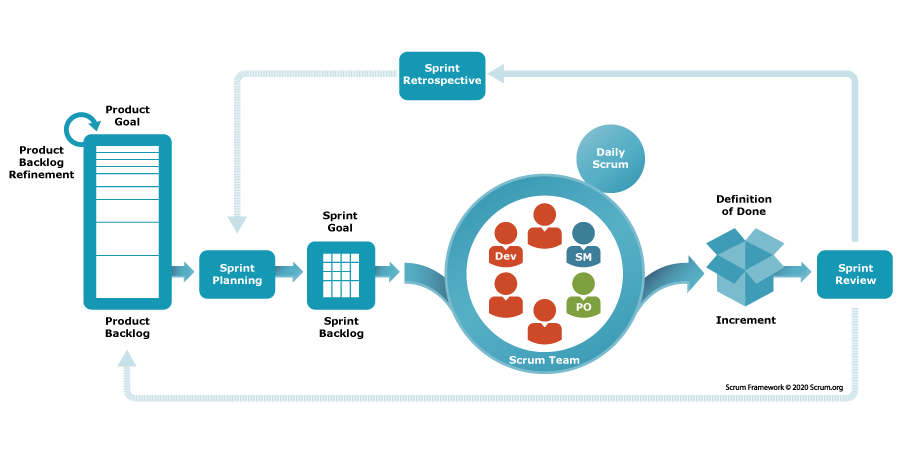
\includegraphics[width=0.9\linewidth]{figures/scrum.png}
    \caption{Schéma du cycle Scrum et de ses principales étapes.}
    \label{fig:scrum_process}
\end{figure}

Les rôles clés définis pour ce projet sont :
\begin{itemize}
    \item \textbf{Product Owner :} Représente les intérêts des utilisateurs finaux et définit les priorités fonctionnelles du backlog.
    \item \textbf{Scrum Master :} Garantit le respect de la méthodologie Scrum, facilite les rituels et élimine les obstacles rencontrés.
    \item \textbf{Équipe de Développement :} Responsable de la réalisation des incréments techniques et de la qualité logicielle.
\end{itemize}

L’équipe Scrum de ce projet est présentée dans le tableau \ref{table:equipe_scrum}.

\begin{table}[H]
\centering
\caption{Équipe Scrum du projet Certif-fun.}
\label{table:equipe_scrum}
\begin{tabular}{|l|l|}
\hline
\textbf{Rôle} & \textbf{Personne en charge} \\ \hline
Product Owner & Pr. LAANAOUI My Driss \\ \hline
Scrum Master & Anas KHAIY \\ \hline
Équipe de Développement & Anas KHAIY \\ \hline
\end{tabular}
\end{table}

\subsection{Planification du projet}
La réalisation de Certif-fun a été structurée en 11 sprints majeurs, permettant une gestion granulaire des complexités techniques de l'IA et des microservices.

\begin{table}[H]
\centering
\caption{Planification détaillée des sprints du projet Certif-fun.}
\label{table:sprints}
\begin{tabular}{|l|p{8cm}|l|}
\hline
\textbf{Sprint} & \textbf{Objectifs et tâches} & \textbf{Livrables} \\ \hline
Sprint 1 & \textbf{Étude préalable et Analyse :} Analyse des besoins, spécifications fonctionnelles et choix de la stack technologique. & Cahier des charges \\ \hline
Sprint 2 & \textbf{Conception (UML et Maquettes) :} Création des diagrammes de cas d'utilisation, de classes et conception des maquettes UI. & Dossier de conception \\ \hline
Sprint 3 & \textbf{Infrastructure Microservices :} Mise en place de l'environnement Docker et des squelettes de services (Spring Boot, FastAPI). & Socle technique \\ \hline
Sprint 4 & \textbf{Réalisation du Frontend (React) :} Création des composants de base, intégration de la charte graphique et mise en place de la navigation. & Interfaces de base \\ \hline
Sprint 5 & \textbf{Sécurité et Authentification :} Développement du système d'authentification centralisé par JWT et gestion des ports (9091-9093). & Module Auth sécurisé \\ \hline
Sprint 6 & \textbf{Gestion des Certifications :} Implémentation des fonctionnalités de gestion des cours et des cycles de certification. & Portails Admin/Formateur \\ \hline
Sprint 7 & \textbf{IA de Proctoring :} Intégration des modèles YOLOv8 et MediaPipe pour la surveillance automatisée en temps réel. & Moteur de surveillance \\ \hline
Sprint 8 & \textbf{Module IA Générative :} Intégration d'Ollama pour la génération automatisée de quiz et de résumés de cours. & Assistant pédagogique IA \\ \hline
Sprint 9 & \textbf{Collaboration et Visioconférence :} Développement de l'espace de réunion virtuelle et communication en temps réel. & Module Visioconférence \\ \hline
Sprint 10 & \textbf{Encadrement et UX :} Système de suivi de progression, filtrage avancé, pagination et optimisation mobile (Responsive). & Interface optimisée \\ \hline
Sprint 11 & \textbf{Tests et Finalisation :} Validation globale, tests de charge, correction des bugs et rédaction du rapport final. & Projet finalisé \\ \hline
\end{tabular}
\end{table}

\subsection{Planification temporelle (Diagramme de Gantt)}
La phase de planification est essentielle dans l'élaboration d'un projet. Elle implique la définition et l'organisation minutieuse des diverses tâches constituant le projet, en évaluant le temps et les ressources requis pour leur accomplissement.

J'ai employé le diagramme de \textbf{Gantt} \cite{ramdani2020ordonnancement}, l'un des outils de planification les plus performants pour illustrer visuellement la progression des diverses tâches qui forment un projet. Dans ce graphique, la colonne de gauche détaille toutes les tâches à réaliser, tandis que la ligne supérieure indique les unités de temps (mois). Chaque tâche est représentée par une barre horizontale dont la position et la longueur représentent la date de début, la durée et la date de fin.

Le projet s'étend du \textbf{15 février au 30 juin}, couvrant l'intégralité du cycle de développement de Certif-fun, comme illustré dans la figure \ref{fig:gantt_certif-fun}.

\begin{figure}[H]
    \centering
    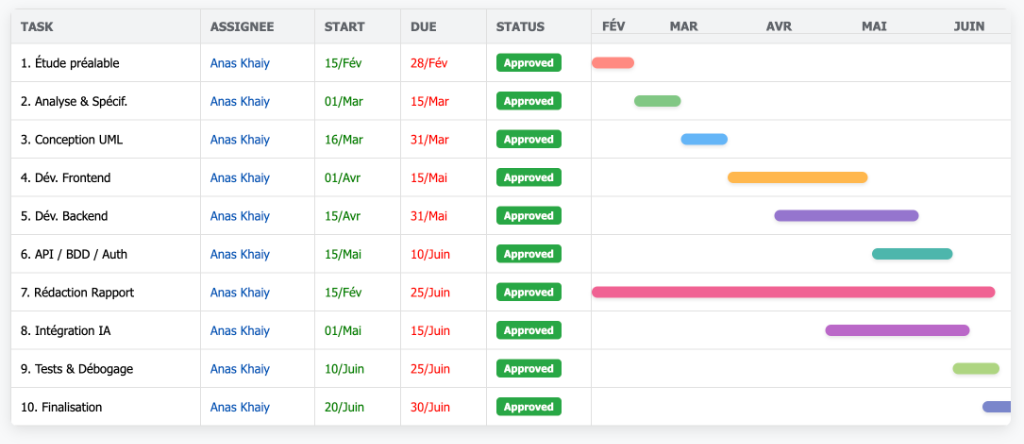
\includegraphics[width=1\linewidth]{figures/gantt_certif-fun.png}
    \caption{Diagramme de Gantt du projet Certif-fun.}
    \label{fig:gantt_certif-fun}
\end{figure}

\section{Conclusion}
En guise de synthèse, ce chapitre a permis de dresser un portrait global du projet \textbf{Certif-fun}. Nous connaissons désormais ses motivations profondes, les insuffisances des solutions actuelles, les objectifs ambitieux à atteindre ainsi que les contraintes techniques et sécuritaires à respecter. Ces éléments permettent de comprendre la pertinence et la finalité de notre travail dans le paysage éducatif actuel.

Malgré une vision claire, certaines difficultés ont été identifiées lors de cette phase initiale, notamment la complexité de l'intégration du traitement vidéo en temps réel au sein d'une architecture microservices et la gestion de la confidentialité des données lors de l'utilisation de modèles d'IA. Ces défis seront abordés avec une attention particulière lors des phases de conception et de réalisation.

Les informations collectées et analysées ici constituent la base solide sur laquelle s'appuiera la suite de notre démarche. Le prochain chapitre détaillera l'\textbf{Étude préliminaire et fonctionnelle}, où nous approfondirons les besoins des utilisateurs, les scénarios métiers et la modélisation des interactions via les diagrammes de cas d'utilisation UML.
